
\documentclass[crop,tikz]{standalone}
\usepackage{tikz}
\newcommand{\red}[1]{\color{red}{\tiny\texttt{#1}}}
\newcommand{\ret}[1]{\color{red}{\footnotesize\texttt{#1}}}
\definecolor{applegreen}{rgb}{0.55, 0.71, 0.0}
\usetikzlibrary{calc,shapes.multipart}
\tikzset{array/.style={rectangle, draw, inner sep=+0pt}}
\tikzset{internal/.style={fill=applegreen, fill opacity=0.2, text opacity=1}}
\tikzset{exit/.style={fill=red, fill opacity=0.2, text opacity=1}}
\tikzset{return/.style={->, color=red, thick}}
\tikzset{call/.style={->, color=applegreen, thick}}
\begin{document}
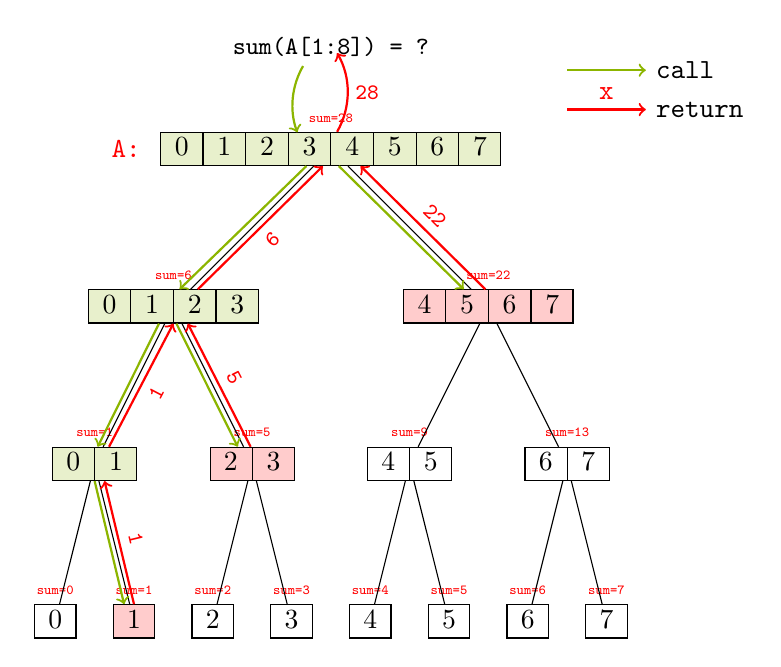
\begin{tikzpicture}
    \node at (-2.6,10) {\color{red}{\texttt{A:}}};
    \node[array,label={above:\red{sum=28}},internal] (root) at (0,10){
        $\begin{array}{c|c|c|c|c|c|c|c}
                0 & 1 & 2 & 3 & 4 & 5 & 6 & 7 \\
            \end{array}$};

    \node[array,label=\red{sum=6},internal] (div1) at (-2,8){
        $\begin{array}{c|c|c|c}
                0 & 1 & 2 & 3 \\
            \end{array}$};

    \node[array, inner sep=+0pt,label=\red{sum=22},exit] (div2) at (2,8){
        $\begin{array}{c|c|c|c}
                4 & 5 & 6 & 7 \\
            \end{array}$};

    \foreach \i in {2,...,3} {
            \pgfmathtruncatemacro{\first}{2*\i}
            \pgfmathtruncatemacro{\second}{2*\i+1}
            \pgfmathtruncatemacro{\s}{4*\i+1}
            \node[array,label=\red{sum=\s}] (upper\i) at (-3+\i*2,6){
                $\begin{array}{c|c}
                        \first & \second \\
                    \end{array}$};
        }

    \node[array,internal,label=\red{sum=1}] (upper0) at (-3,6){
        $\begin{array}{c|c}
                0 & 1 \\
            \end{array}$};

    \node[array,exit,label=\red{sum=5}] (upper1) at (-1,6){
        $\begin{array}{c|c}
                2 & 3 \\
            \end{array}$};

    \foreach \i in {0,2,3,...,7} {
            \node[array,label=\red{sum=\i}] (bottom\i) at (-3.5+\i,4) {
                $\begin{array}{c}
                        \i \\
                    \end{array}$};
        }

    \node[array,exit,label=\red{sum=1}] (bottom1) at (-2.5,4){
        $\begin{array}{c}
                1 \\
            \end{array}$};

    \draw[-]  (root) -- (div1);
    \draw[-]  (root) -- (div2);
    \draw[-]  (div1) -- (upper0);
    \draw[-]  (div1) -- (upper1);
    \draw[-]  (div2) -- (upper2);
    \draw[-]  (div2) -- (upper3);

    \foreach \i in {0,...,3} {
            \pgfmathtruncatemacro{\left}{2*\i}
            \pgfmathtruncatemacro{\right}{2*\i+1}
            \draw[-]  (upper\i) -- (bottom\left);
            \draw[-]  (upper\i) -- (bottom\right);
        }

    \draw[call] (root.215) -- (div1.70);
    \draw[call] (root.295) -- (div2.145);
    \draw[call] (div1.230) -- (upper0.80);
    \draw[call] (div1.280) -- (upper1.130);
    \draw[call] (upper0.270) -- (bottom1.120);

    \draw[return] (bottom1.90) -- node[sloped,above]{\ret{1}} (upper0.300);
    \draw[return] (upper0.50) -- node[sloped,below]{\ret{1}} (div1.270);
    \draw[return] (upper1.95) -- node[sloped,above]{\ret{5}} (div1.310);
    \draw[return] (div1.35) -- node[sloped,below]{\ret{6}} (root.245);

    \draw[return] (div2.100) -- node[sloped,above]{\ret{22}} (root.330);

    \node (query) at (0,11.3){\small\texttt{sum(A[1:8]) = ?}};

    \draw[call] (query.215) arc[radius=1, start angle=150, end angle=200] (root);
    \draw[return] (root.70) arc[radius=1, start angle=-30, end angle=30] node[sloped,right,yshift=-0.5cm,xshift=0.1cm]{\ret{28}} (query);

    \draw[call] (3,11) -- (4,11) node[text=black,right]{\texttt{call}};
    \draw[return](3,10.5) -- node[sloped,above]{\texttt{x}}  (4,10.5) node[text=black,right]{\texttt{return}};

\end{tikzpicture}
\end{document}